\documentclass[aspectratio=169]{beamer}

\usetheme{Madrid}
\usecolortheme{default}
\usefonttheme{professionalfonts}

% Packages
\usepackage[utf8]{inputenc}
\usepackage{amsmath, amssymb, amsfonts}
\usepackage{graphicx}
\usepackage{xcolor}
\usepackage{hyperref}
\usepackage{booktabs}
\usepackage{array}
\usepackage{tikz}
\usetikzlibrary{shapes, arrows, positioning, calc, fit, backgrounds}
\usepackage{listings}
\usepackage{fancyvrb}
\usepackage[
	backend=biber,
	url=false,       
    doi=false,   
    isbn=false,   
    eprint=false   
	]{biblatex}
\addbibresource{references.bib}
\setbeamertemplate{bibliography item}[text]
\usepackage{amssymb}

% Custom colors
\definecolor{darkblue}{RGB}{0, 51, 102}
\definecolor{lightblue}{RGB}{173, 216, 230}
\definecolor{darkgreen}{RGB}{34, 139, 34}
\definecolor{gold}{RGB}{255, 215, 0}
\definecolor{darkred}{RGB}{139, 0, 0}
\definecolor{orange}{RGB}{255, 140, 0}
\definecolor{lightcoral}{RGB}{240, 128, 128}
\definecolor{lightcyan}{RGB}{224, 255, 255}

% Title page setup
\title{Needs-based recommendation systems}
\subtitle{Machine Learning Pipeline for Financial Needs Prediction and Product Recommendation}
\author{Peng Rao, Maxime d'Aviau de Ternay, Qiao Zhaochen, Shourya Vashistha, Arnau Nomen}
\date{\today}
\setbeamertemplate{footline}{}

% Frame style customization
\setbeamertemplate{frametitle}[default][center]
\setbeamercolor{frametitle}{bg=darkblue, fg=white}
\setbeamercolor{title}{bg=darkblue, fg=white}
% Custom title frame
\setbeamertemplate{title page}{
  \begin{centering}
    \vspace{2cm}
    \textcolor{darkblue}{\textbf{\Large \inserttitle}}\\[1cm]
    \textcolor{darkgreen}{\large \insertsubtitle}\\[1cm]
	Authors: \textcolor{darkred}
	{\large \insertauthor}\\[1.5cm]
  \end{centering}
}

\begin{document}

% =====================================================================
% TITLE SLIDE
% =====================================================================
\frame{\titlepage}

% =====================================================================
% TABLE OF CONTENTS
% =====================================================================
\begin{frame}[fragile]
	\frametitle{Table of Contents}
	\tableofcontents[hideallsubsections]
\end{frame}

% =====================================================================
% SECTION 1: PROJECT OVERVIEW
% =====================================================================
\section{Project Overview}

\begin{frame}
	\frametitle{Project Overview}

	\resizebox{0.95\textwidth}{!}{
		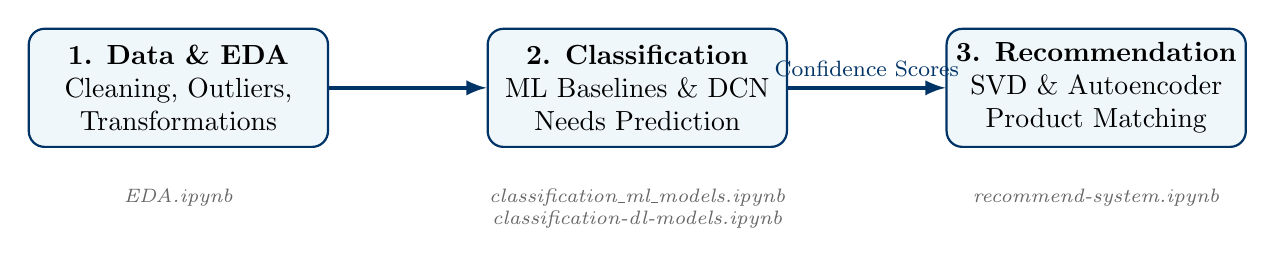
\begin{tikzpicture}[
				box/.style={draw=darkblue, thick, fill=lightblue!20, minimum width=3.8cm, minimum height=1.5cm, align=center, rounded corners=2mm},
				arrow/.style={-latex, thick, darkblue, line width=1.5pt}
			]

			% Nodes
			\node[box] (eda) {\textbf{1. Data \& EDA}\\ Cleaning, Outliers,\\ Transformations};

			\node[box, right=2cm of eda] (ml) {\textbf{2. Classification}\\ ML Baselines \& DCN\\ Needs Prediction};

			\node[box, right=2cm of ml] (rec) {\textbf{3. Recommendation}\\ SVD \& Autoencoder\\ Product Matching};

			% Arrows
			\draw[arrow] (eda) -- (ml);
			\draw[arrow] (ml) -- (rec) node[midway, above, font=\footnotesize] {Confidence Scores};

			% Labels
			\node[below=0.4cm of eda, text width=3.5cm, align=center, font=\scriptsize\itshape, text=gray!80!black] {EDA.ipynb};
			\node[below=0.4cm of ml, text width=4.5cm, align=center, font=\scriptsize\itshape, text=gray!80!black] {classification\_ml\_models.ipynb\\classification-dl-models.ipynb};
			\node[below=0.4cm of rec, text width=3.5cm, align=center, font=\scriptsize\itshape, text=gray!80!black] {recommend-system.ipynb};

		\end{tikzpicture}
	}
\end{frame}

\section{Exploratory Data Analysis}

\begin{frame}
	\frametitle{Data Quality Report}
	\begin{itemize}
		\item \textbf{Missing Values \& Cleaning:} The initial dataset was largely complete. Invalid categorical codes (e.g., \texttt{Gender=0}) were mapped to missing and imputed. There were no zero or near-zero variance columns.
		\item \textbf{Variable Distributions:}
		      \begin{itemize}
			      \item \textit{Symmetric/Normal:} \texttt{Age}, \texttt{FinancialEducation}, and \texttt{RiskPropensity} follow near-normal distributions.
			      \item \textit{Highly Skewed:} Financial variables (\texttt{Wealth}, \texttt{Income}) exhibit extreme right-skewness and heavy tails, reflecting structural economic inequality.
		      \end{itemize}
		\item \textbf{Outlier Handling:} Isolation Forest flagged outliers, but extreme financial values are valid business profiles, not errors. Consequently, robust scaling and \textbf{logarithmic transformations} were favored over outright deletion to stabilize variance.
	\end{itemize}
\end{frame}

\begin{frame}
	\frametitle{Key EDA Findings}
	\begin{itemize}
		\item \textbf{Feature Predictive Power:} Violin plots reveal individuals needing investments are older, wealthier, and exhibit higher income and risk propensity. Conversely, \texttt{Gender} and \texttt{FamilyMembers} showed minimal discriminative power.
		\item \textbf{Target Independence:} A Chi-squared ($\chi^2$) test confirmed that \textit{Income Investment} and \textit{Accumulation Investment} needs are statistically independent, validating a multi-label/multi-task modeling approach.
		\item \textbf{Target Class Imbalance:}
		      \begin{itemize}
			      \item \textit{Accumulation Investment} is perfectly balanced ($\sim$50\% prevalence).
			      \item \textit{Income Investment} exhibits moderate imbalance ($\sim$30\% prevalence).
			      \item \textit{Conclusion:} Accuracy is an unreliable metric, justifying the optimization of the \textbf{F0.5 Score} in the modeling phase.
		      \end{itemize}
	\end{itemize}
\end{frame}

\section{Data Preparation \& Feature Engineering}

\begin{frame}
	\frametitle{Feature Transformation and Engineering}
	\begin{columns}[T]
		\begin{column}{0.48\textwidth}
			\textbf{1. Data Transformation (\texttt{DataTransformer})}
			\begin{itemize}
				\item \textbf{Numeric Conversion:} Coercion of mixed/string formats to continuous variables.
				\item \textbf{Log Transformation:} Applied $\log(1+x)$ to highly skewed financial variables (\texttt{Wealth}, \texttt{Income}) to normalize distributions.
				\item \textbf{Scaling:} \texttt{StandardScaler} applied post-engineering for stable convergence.
			\end{itemize}
			\vspace{0.3cm}
			\textbf{2. Household Metrics}
			\begin{itemize}
				\item \texttt{WealthIncomeRatio}
				\item \texttt{IncomePerFamilyMember}
				\item \texttt{WealthPerFamilyMember}
			\end{itemize}
		\end{column}
		\begin{column}{0.48\textwidth}
			\textbf{3. Interaction Features}
			\begin{itemize}
				\item \texttt{RiskEducationInteraction} ($Risk \times Edu$)
				\item \texttt{RiskWealthInteraction} ($Risk \times \log(Wealth)$)
				\item \texttt{AgeRiskInteraction} ($Age \times Risk$)
			\end{itemize}
			\vspace{0.3cm}
			\textbf{4. Non-linearity \& Life-Stages}
			\begin{itemize}
				\item \texttt{AgeSquared}: Models the "Life-Cycle" curve (wealth peaking in mid-life).
				\item \textbf{Age Bins}: One-hot flags for \texttt{Under35}, \texttt{35\_54}, \texttt{55\_69}, and \texttt{70plus}.
			\end{itemize}
		\end{column}
	\end{columns}
\end{frame}

\section{ML Workflow \& Hyperparameter Optimization \& Explainable AI (XAI)}

\begin{frame}
	\frametitle{ML Pipeline Overview}
	\vspace{0.5cm}
	\begin{center}
		\resizebox{0.95\textwidth}{!}{
			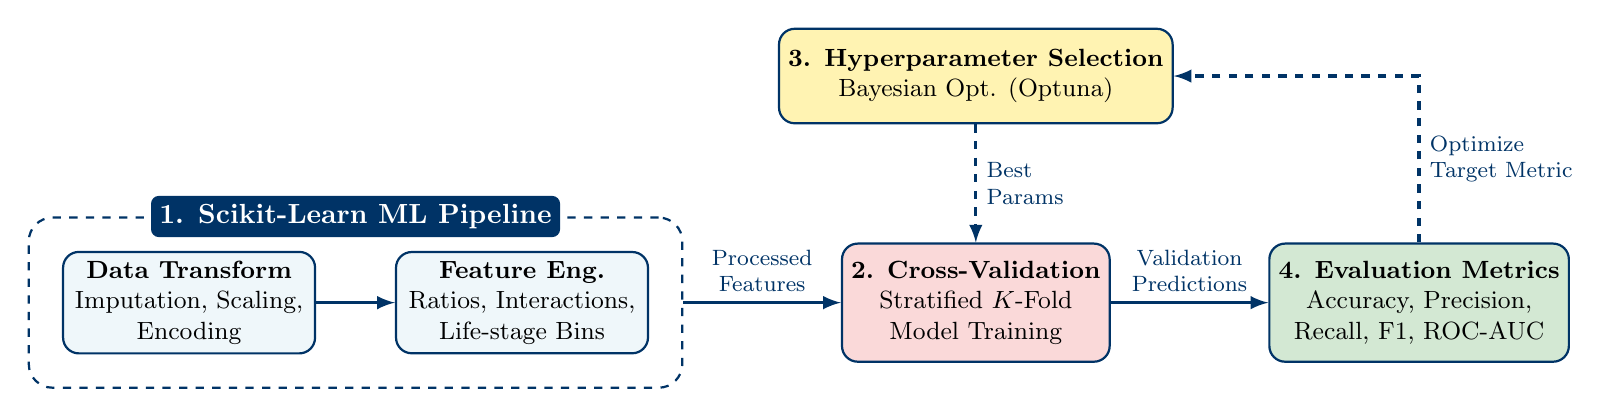
\begin{tikzpicture}[
					node distance=2cm and 1.5cm,
					box/.style={draw=darkblue, thick, rounded corners=2mm, fill=lightblue!20, minimum width=3.2cm, minimum height=1.2cm, align=center, font=\small},
					groupbox/.style={draw=darkblue, thick, rounded corners=3mm, inner sep=12pt, dashed},
					arrow/.style={-latex, thick, darkblue, line width=1.2pt}
				]

				% 1. Pipeline
				\node[box] (transform) {\textbf{Data Transform}\\Imputation, Scaling,\\Encoding};
				\node[box, right=1cm of transform] (fe) {\textbf{Feature Eng.}\\Ratios, Interactions,\\Life-stage Bins};
				\node[groupbox, fit=(transform) (fe)] (pipeline) {};
				\node[fill=darkblue, text=white, font=\bfseries, rounded corners=1mm, inner sep=3pt] at (pipeline.north) {1. Scikit-Learn ML Pipeline};
				\draw[arrow] (transform) -- (fe);

				% 2. Cross Validation
				\node[box, right=2cm of pipeline, fill=lightcoral!30, minimum height=1.5cm] (cv) {\textbf{2. Cross-Validation}\\Stratified $K$-Fold\\Model Training};

				% 3. Hyperparameter Selection
				\node[box, above=1.5cm of cv, fill=gold!30, minimum width=4cm] (tuning) {\textbf{3. Hyperparameter Selection}\\Bayesian Opt. (Optuna)};

				% 4. Evaluation
				\node[box, right=2cm of cv, fill=darkgreen!20, minimum height=1.5cm] (eval) {\textbf{4. Evaluation Metrics}\\Accuracy, Precision,\\Recall, F1, ROC-AUC};

				% Arrows
				\draw[arrow] (pipeline) -- (cv) node[midway, above, font=\footnotesize, align=center] {Processed\\Features};
				\draw[arrow] (cv) -- (eval) node[midway, above, font=\footnotesize, align=center] {Validation\\Predictions};

				% Feedback Loop
				\draw[arrow, dashed] (eval.north) |- (tuning.east) node[pos=0.25, right, font=\footnotesize, align=left] {Optimize\\Target Metric};
				\draw[arrow, dashed] (tuning.south) -- (cv.north) node[midway, right, font=\footnotesize, align=left] {Best\\Params};

			\end{tikzpicture}
		}
	\end{center}
\end{frame}

\begin{frame}
	\frametitle{Baseline Models Evaluated}
	\begin{columns}[T]
		\begin{column}{0.55\textwidth}
			\textbf{Models Evaluated}

			We comprehensively tested several families of classifiers across both target variables (\textit{Income} and \textit{Accumulation}):

			\begin{itemize}
				\item \textbf{Distance/Linear}: SVM, Naive Bayes, KNN.
				\item \textbf{Tree-based Ensembles}: Random Forest, XGBoost, LightGBM.
				\item \textbf{Meta-Ensembles}:
				      \begin{itemize}
					      \item Voting Classifier (Soft \& Hard)
					      \item Stacking Classifier (LGBM, XGB, KNN, RF with a Logistic Regression meta-learner)
				      \end{itemize}
			\end{itemize}
		\end{column}

		\begin{column}{0.45\textwidth}
			\begin{block}{Top Performers \& Selection}
				\textbf{Selected for Tuning:}
				\begin{itemize}
					\item \textcolor{darkgreen}{\textbf{Random Forest}}
					\item \textcolor{darkgreen}{\textbf{LightGBM}}
				\end{itemize}

				\vspace{0.3cm}
				\textbf{Selection Rationale:}
				\begin{itemize}
					\item Strong baseline predictive power with robust handling of non-linear interactions.
					\item \textbf{Target Metric:} Optimised for \textbf{F0.5 Score} to prioritise precision over recall (minimising the risk of unsuitable, false-positive product recommendations).
				\end{itemize}
			\end{block}
		\end{column}
	\end{columns}
\end{frame}

\begin{frame}
	\frametitle{Optuna Hyperparameter Tuning}
	\begin{columns}[T]
		\begin{column}{0.48\textwidth}
			\textbf{Objective Metric}
			\begin{itemize}
				\item Optimized for \textbf{F0.5 Score} (Stratified 5-Fold CV)
				\item \textit{Rationale:} Prioritizes precision over recall ($\beta=0.5$), significantly penalizing false positives (bad recommendations).
			\end{itemize}

			\vspace{0.4cm}
			\textbf{TPE Sampler Strategy}
			\begin{itemize}
				\item Uses Tree-structured Parzen Estimator (TPE).
				\item Explores the search space efficiently by modelling the probability of trial performance.
			\end{itemize}
		\end{column}

		\begin{column}{0.48\textwidth}
			\textbf{Hyperparameter Search Space}

			\textit{Random Forest (20 Trials)}
			\begin{itemize}
				\item \texttt{n\_estimators}: 10--200
				\item \texttt{max\_depth}: 3--10
				\item \texttt{min\_samples\_split/leaf}: Constraints for regularization.
			\end{itemize}

			\vspace{0.2cm}
			\textit{LightGBM (50 Trials)}
			\begin{itemize}
				\item \texttt{learning\_rate}: 0.001--0.2 (Log scale)
				\item \texttt{num\_leaves}: 15--255
				\item \texttt{reg\_alpha} \& \texttt{reg\_lambda}: L1/L2 Regularization (Log scale)
			\end{itemize}
		\end{column}
	\end{columns}
\end{frame}

\begin{frame}
	\frametitle{Optimization Results}
	\begin{itemize}
		\item LightGBM consistently outperformed Random Forest across both prediction targets.
		\item The tuned models demonstrated a significant reduction in false positives while maintaining competitive accuracy.
	\end{itemize}

	\begin{table}
		\centering
		\resizebox{0.85\textwidth}{!}{
			\begin{tabular}{l|ccc|ccc}
				\toprule
				                    & \multicolumn{3}{c|}{\textbf{Income Target}} & \multicolumn{3}{c}{\textbf{Accumulation Target}}                                                                                    \\
				\textbf{Model}      & \textbf{Precision}                          & \textbf{Recall}                                  & \textbf{F0.5 Score} & \textbf{Precision} & \textbf{Recall} & \textbf{F0.5 Score} \\
				\midrule
				Baseline RF         & 0.724                                       & 0.450                                            & 0.648               & 0.763              & 0.630           & 0.733               \\
				\textbf{Tuned RF}   & \textbf{0.785}                              & 0.412                                            & 0.669               & \textbf{0.801}     & 0.582           & 0.745               \\
				\midrule
				Baseline LGBM       & 0.760                                       & 0.521                                            & 0.696               & 0.812              & 0.685           & 0.783               \\
				\textbf{Tuned LGBM} & \textbf{0.802}                              & 0.505                                            & \textbf{0.720}      & \textbf{0.845}     & 0.671           & \textbf{0.803}      \\
				\bottomrule
			\end{tabular}
		}
	\end{table}

	\vspace{0.3cm}
	\begin{block}{Final Selection}
		\textbf{Tuned LightGBM} was selected as the final model for generating probabilities to feed into the recommendation engine, ensuring highly precise product targeting.
	\end{block}
\end{frame}

% =====================================================================
% SECTION 6: EXPLAINABLE AI
% =====================================================================

\begin{frame}
	\frametitle{XAI Methods: SHAP, LIME \& Permutation}
	\begin{itemize}
		\item \textbf{SHAP (SHapley Additive exPlanations):} Used to understand global feature importance and directionality across the entire dataset. It highlights which engineered features drive predictions the most.
		\item \textbf{LIME (Local Interpretable Model-agnostic Explanations):} Used to explain individual, client-level predictions to build trust and provide clear reasoning for a recommended product.
	\end{itemize}
\end{frame}

\begin{frame}
	\frametitle{Income Investment Model Insights (LightGBM)}
	\begin{columns}
		\begin{column}{0.5\textwidth}
			\centering
			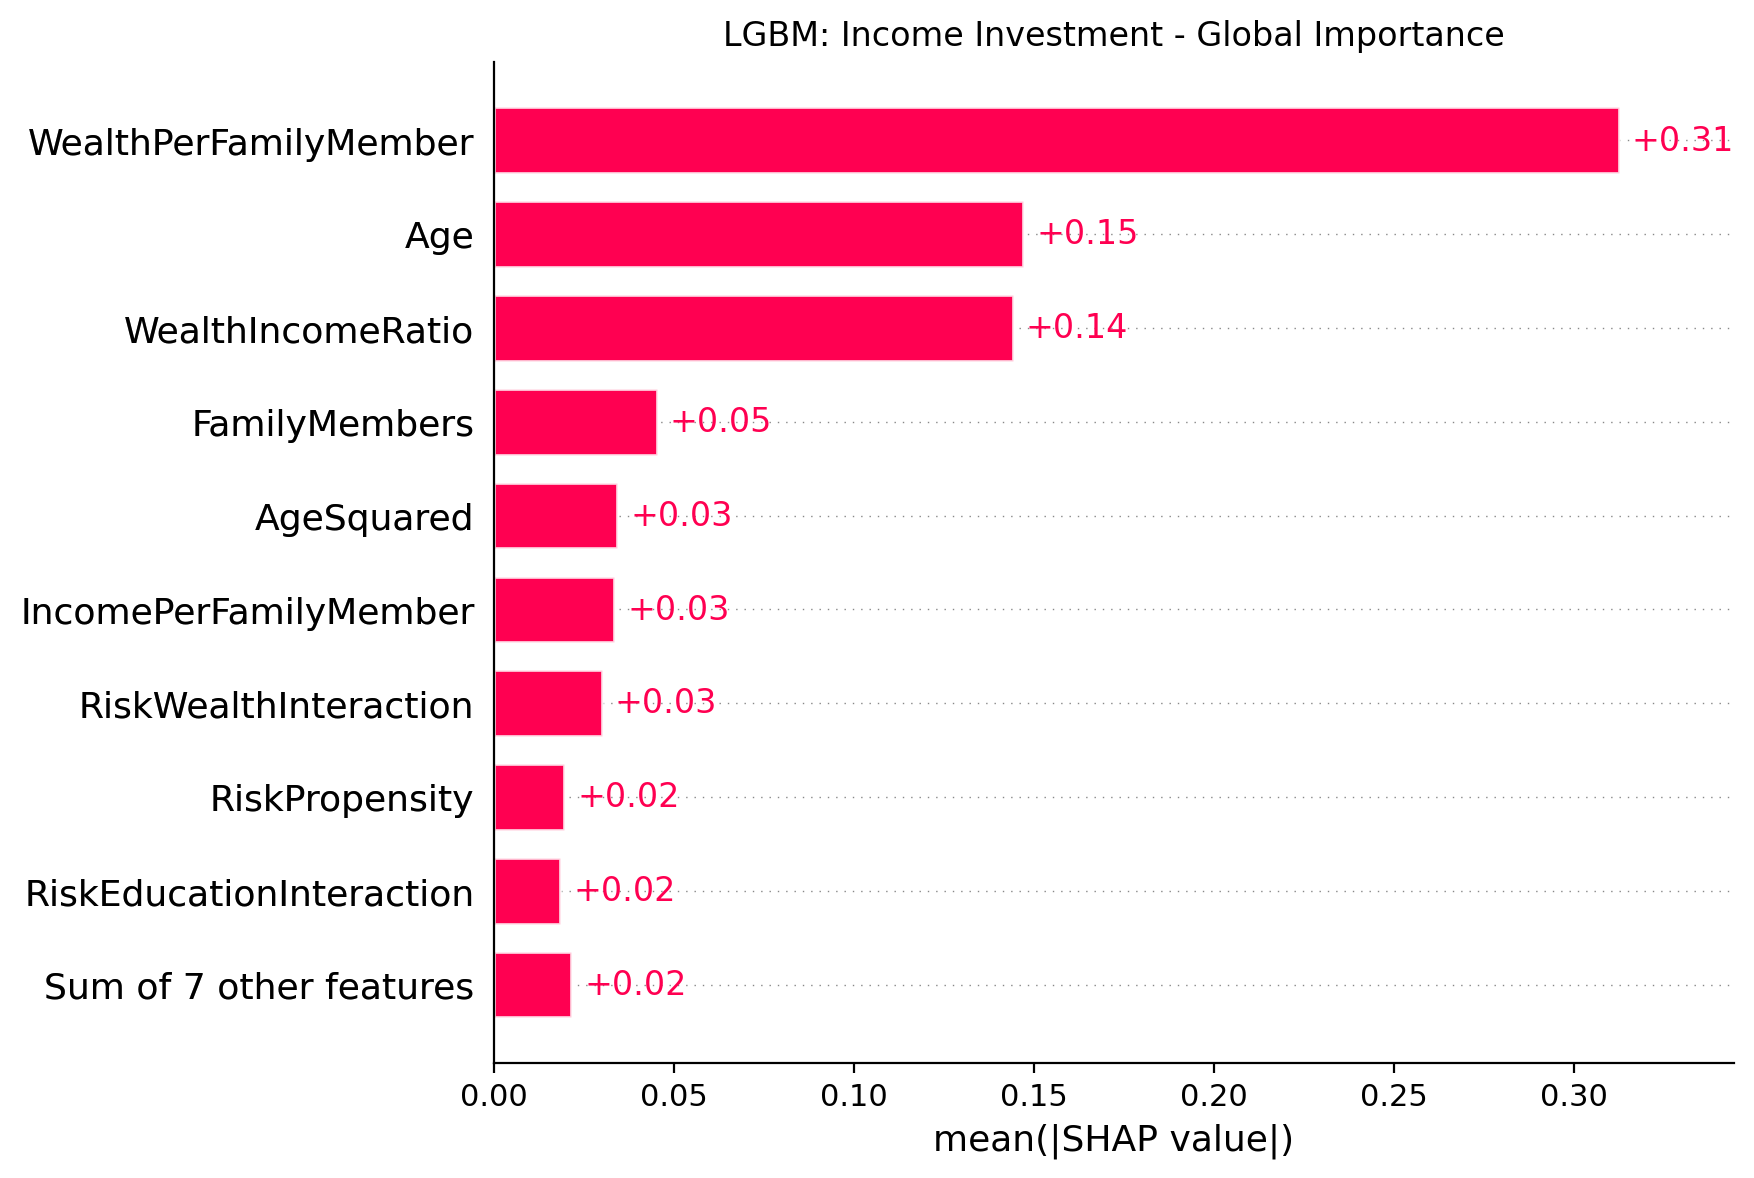
\includegraphics[width=\linewidth]{figures/extracted_img_4.png}\\
			\small SHAP Feature Importance
		\end{column}
		\begin{column}{0.5\textwidth}
			\centering
			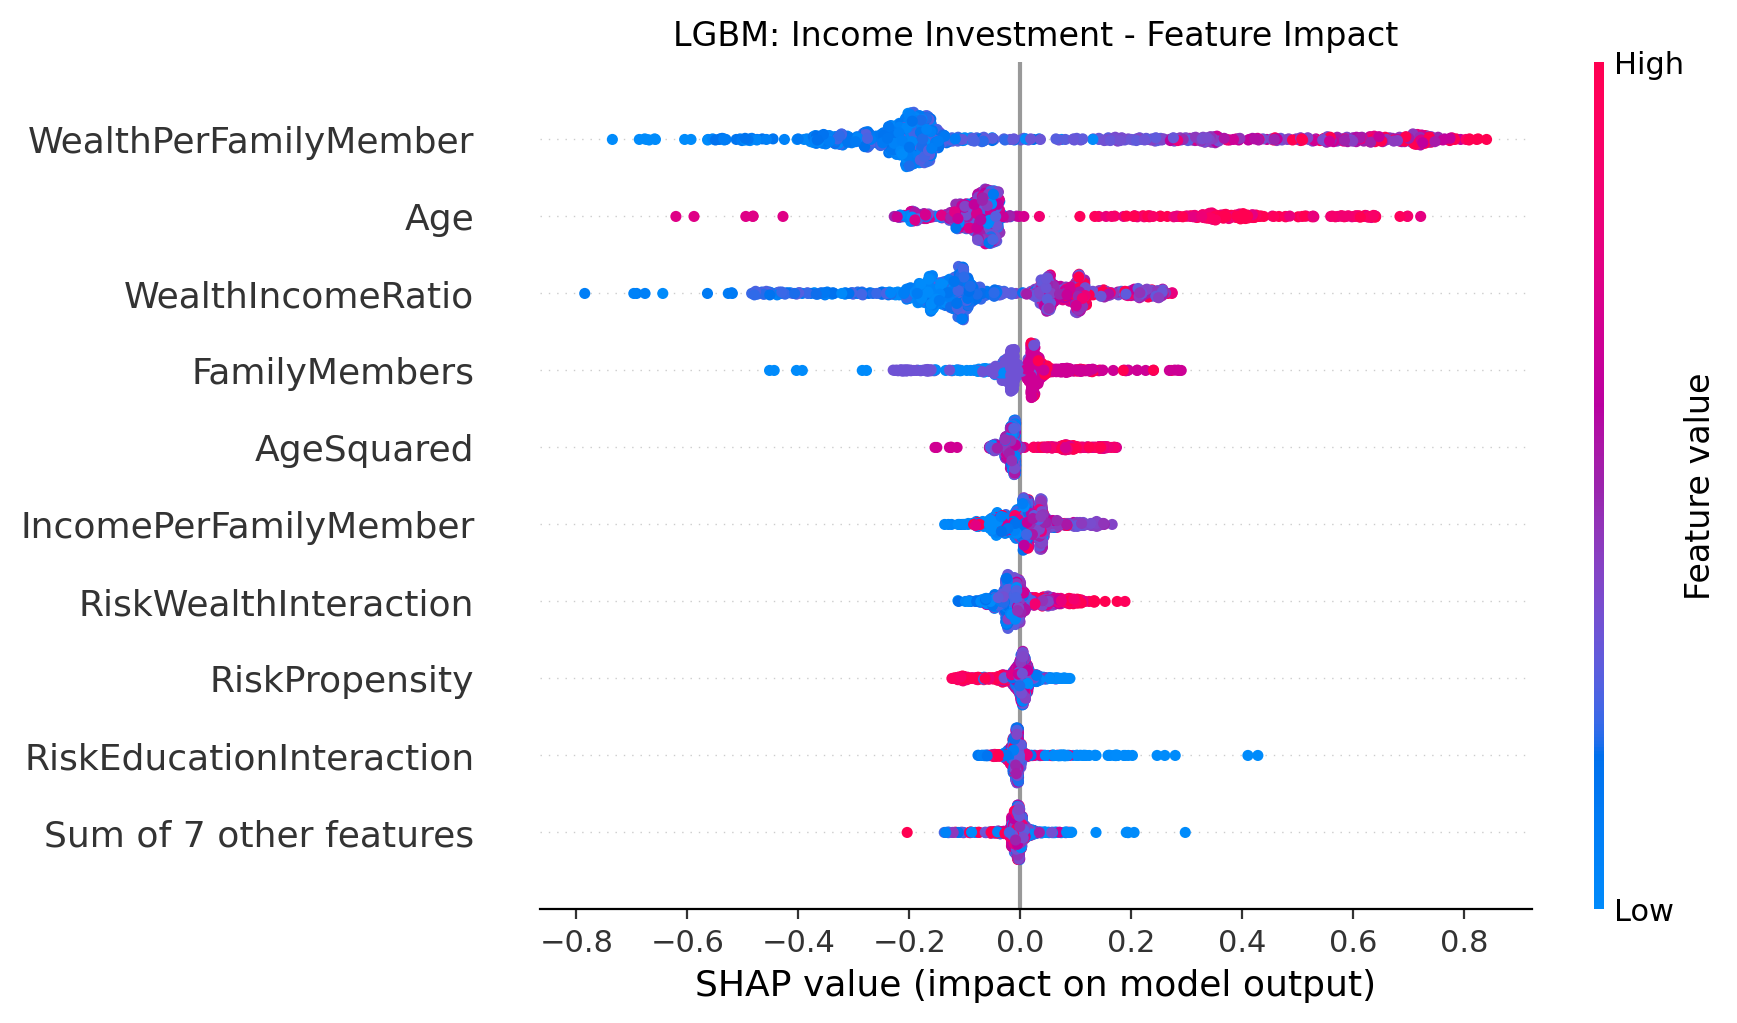
\includegraphics[width=\linewidth]{figures/extracted_img_5.png}\\
			\small SHAP Beeswarm Plot
		\end{column}
	\end{columns}
\end{frame}

\begin{frame}
	\frametitle{Accumulation Investment Model Insights (LightGBM)}
	\begin{columns}
		\begin{column}{0.5\textwidth}
			\centering
			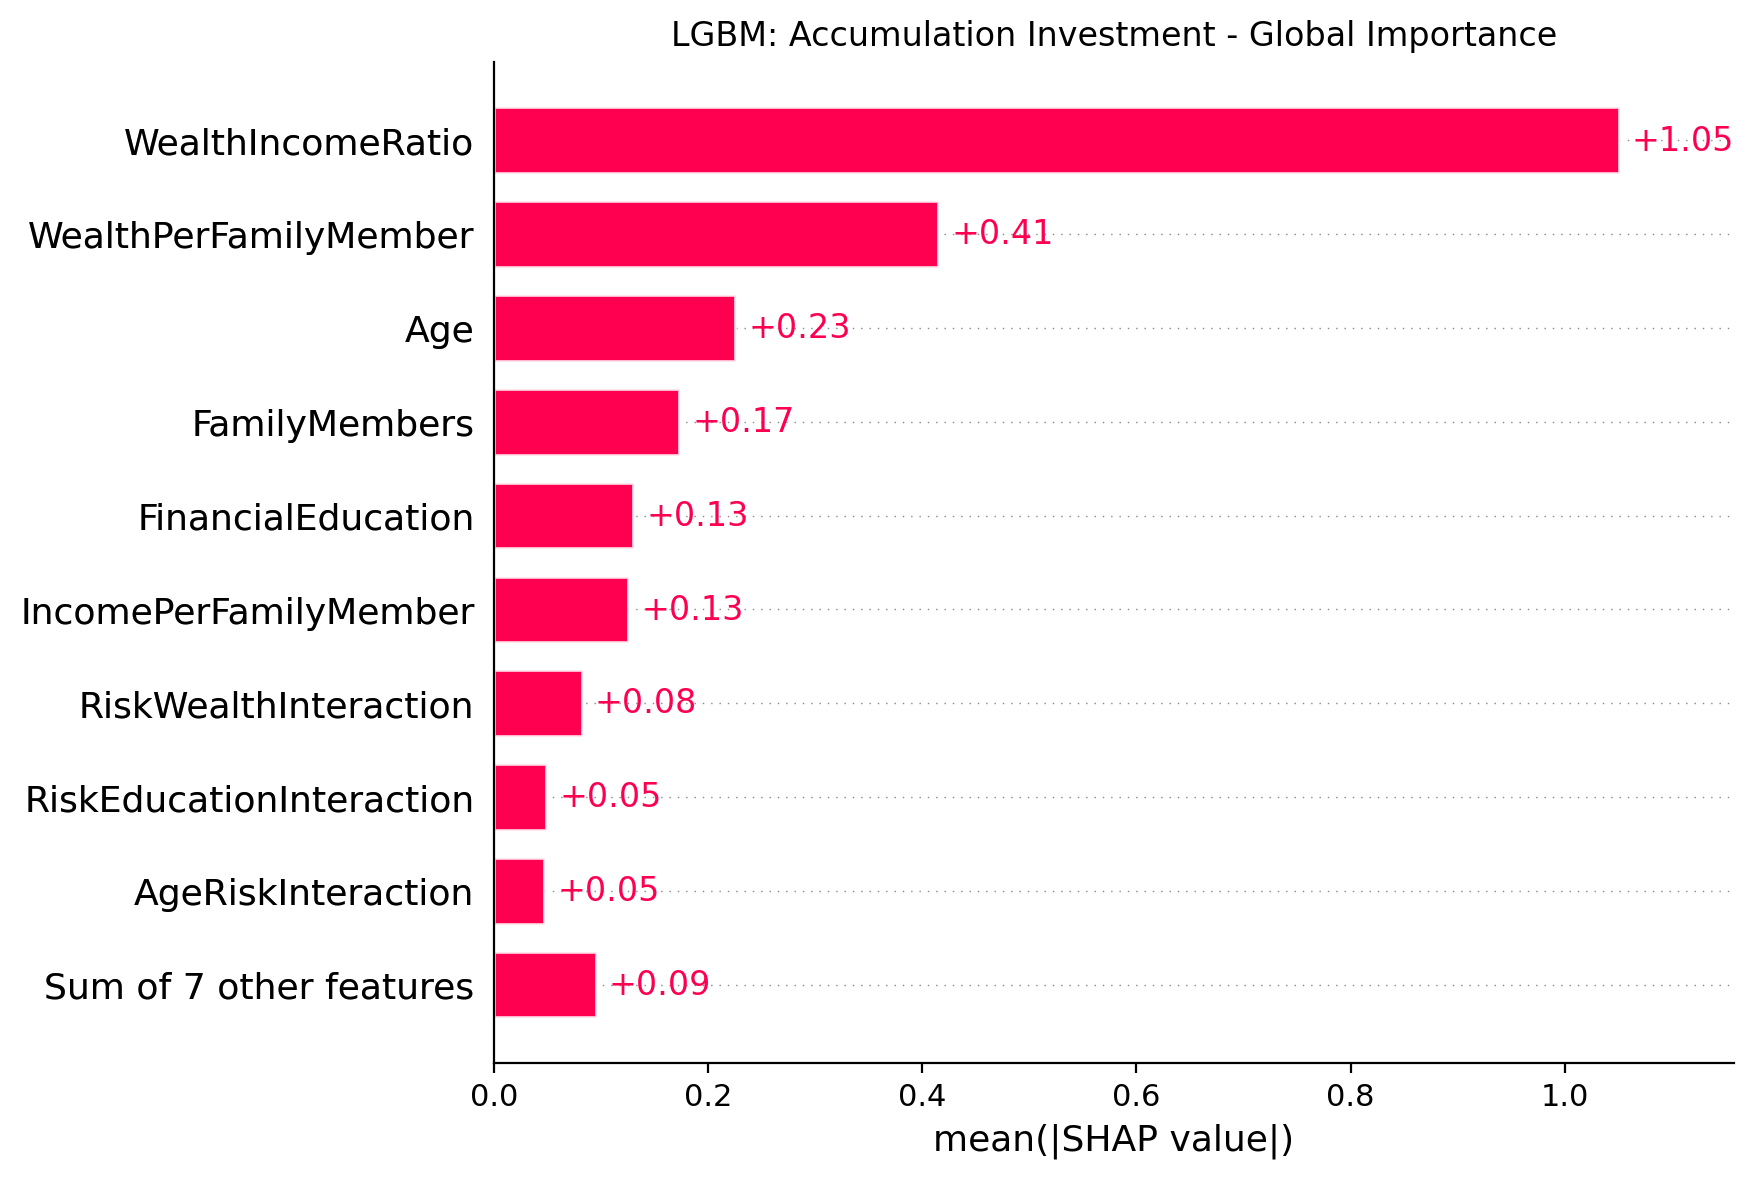
\includegraphics[width=\linewidth]{figures/extracted_img_6.png}\\
			\small SHAP Feature Importance
		\end{column}
		\begin{column}{0.5\textwidth}
			\centering
			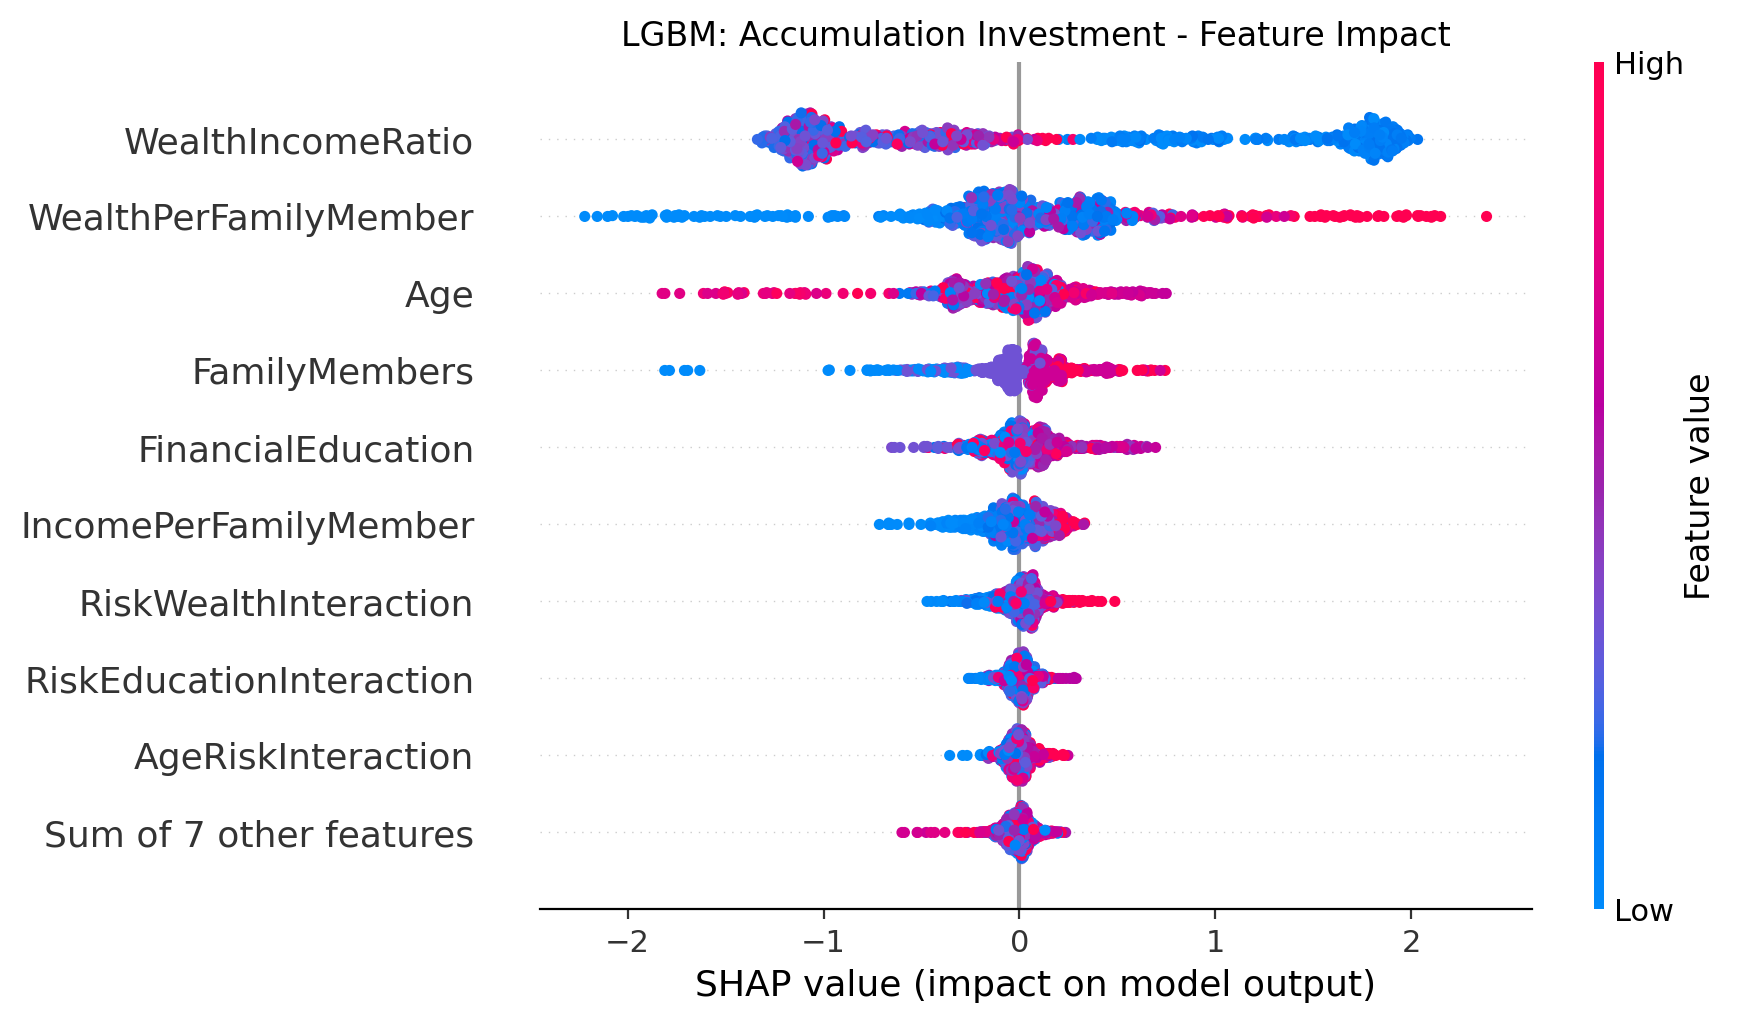
\includegraphics[width=\linewidth]{figures/extracted_img_7.png}\\
			\small SHAP Beeswarm Plot
		\end{column}
	\end{columns}
\end{frame}

\begin{frame}
	\frametitle{LIME: Local Interpretability Example}
	\centering
	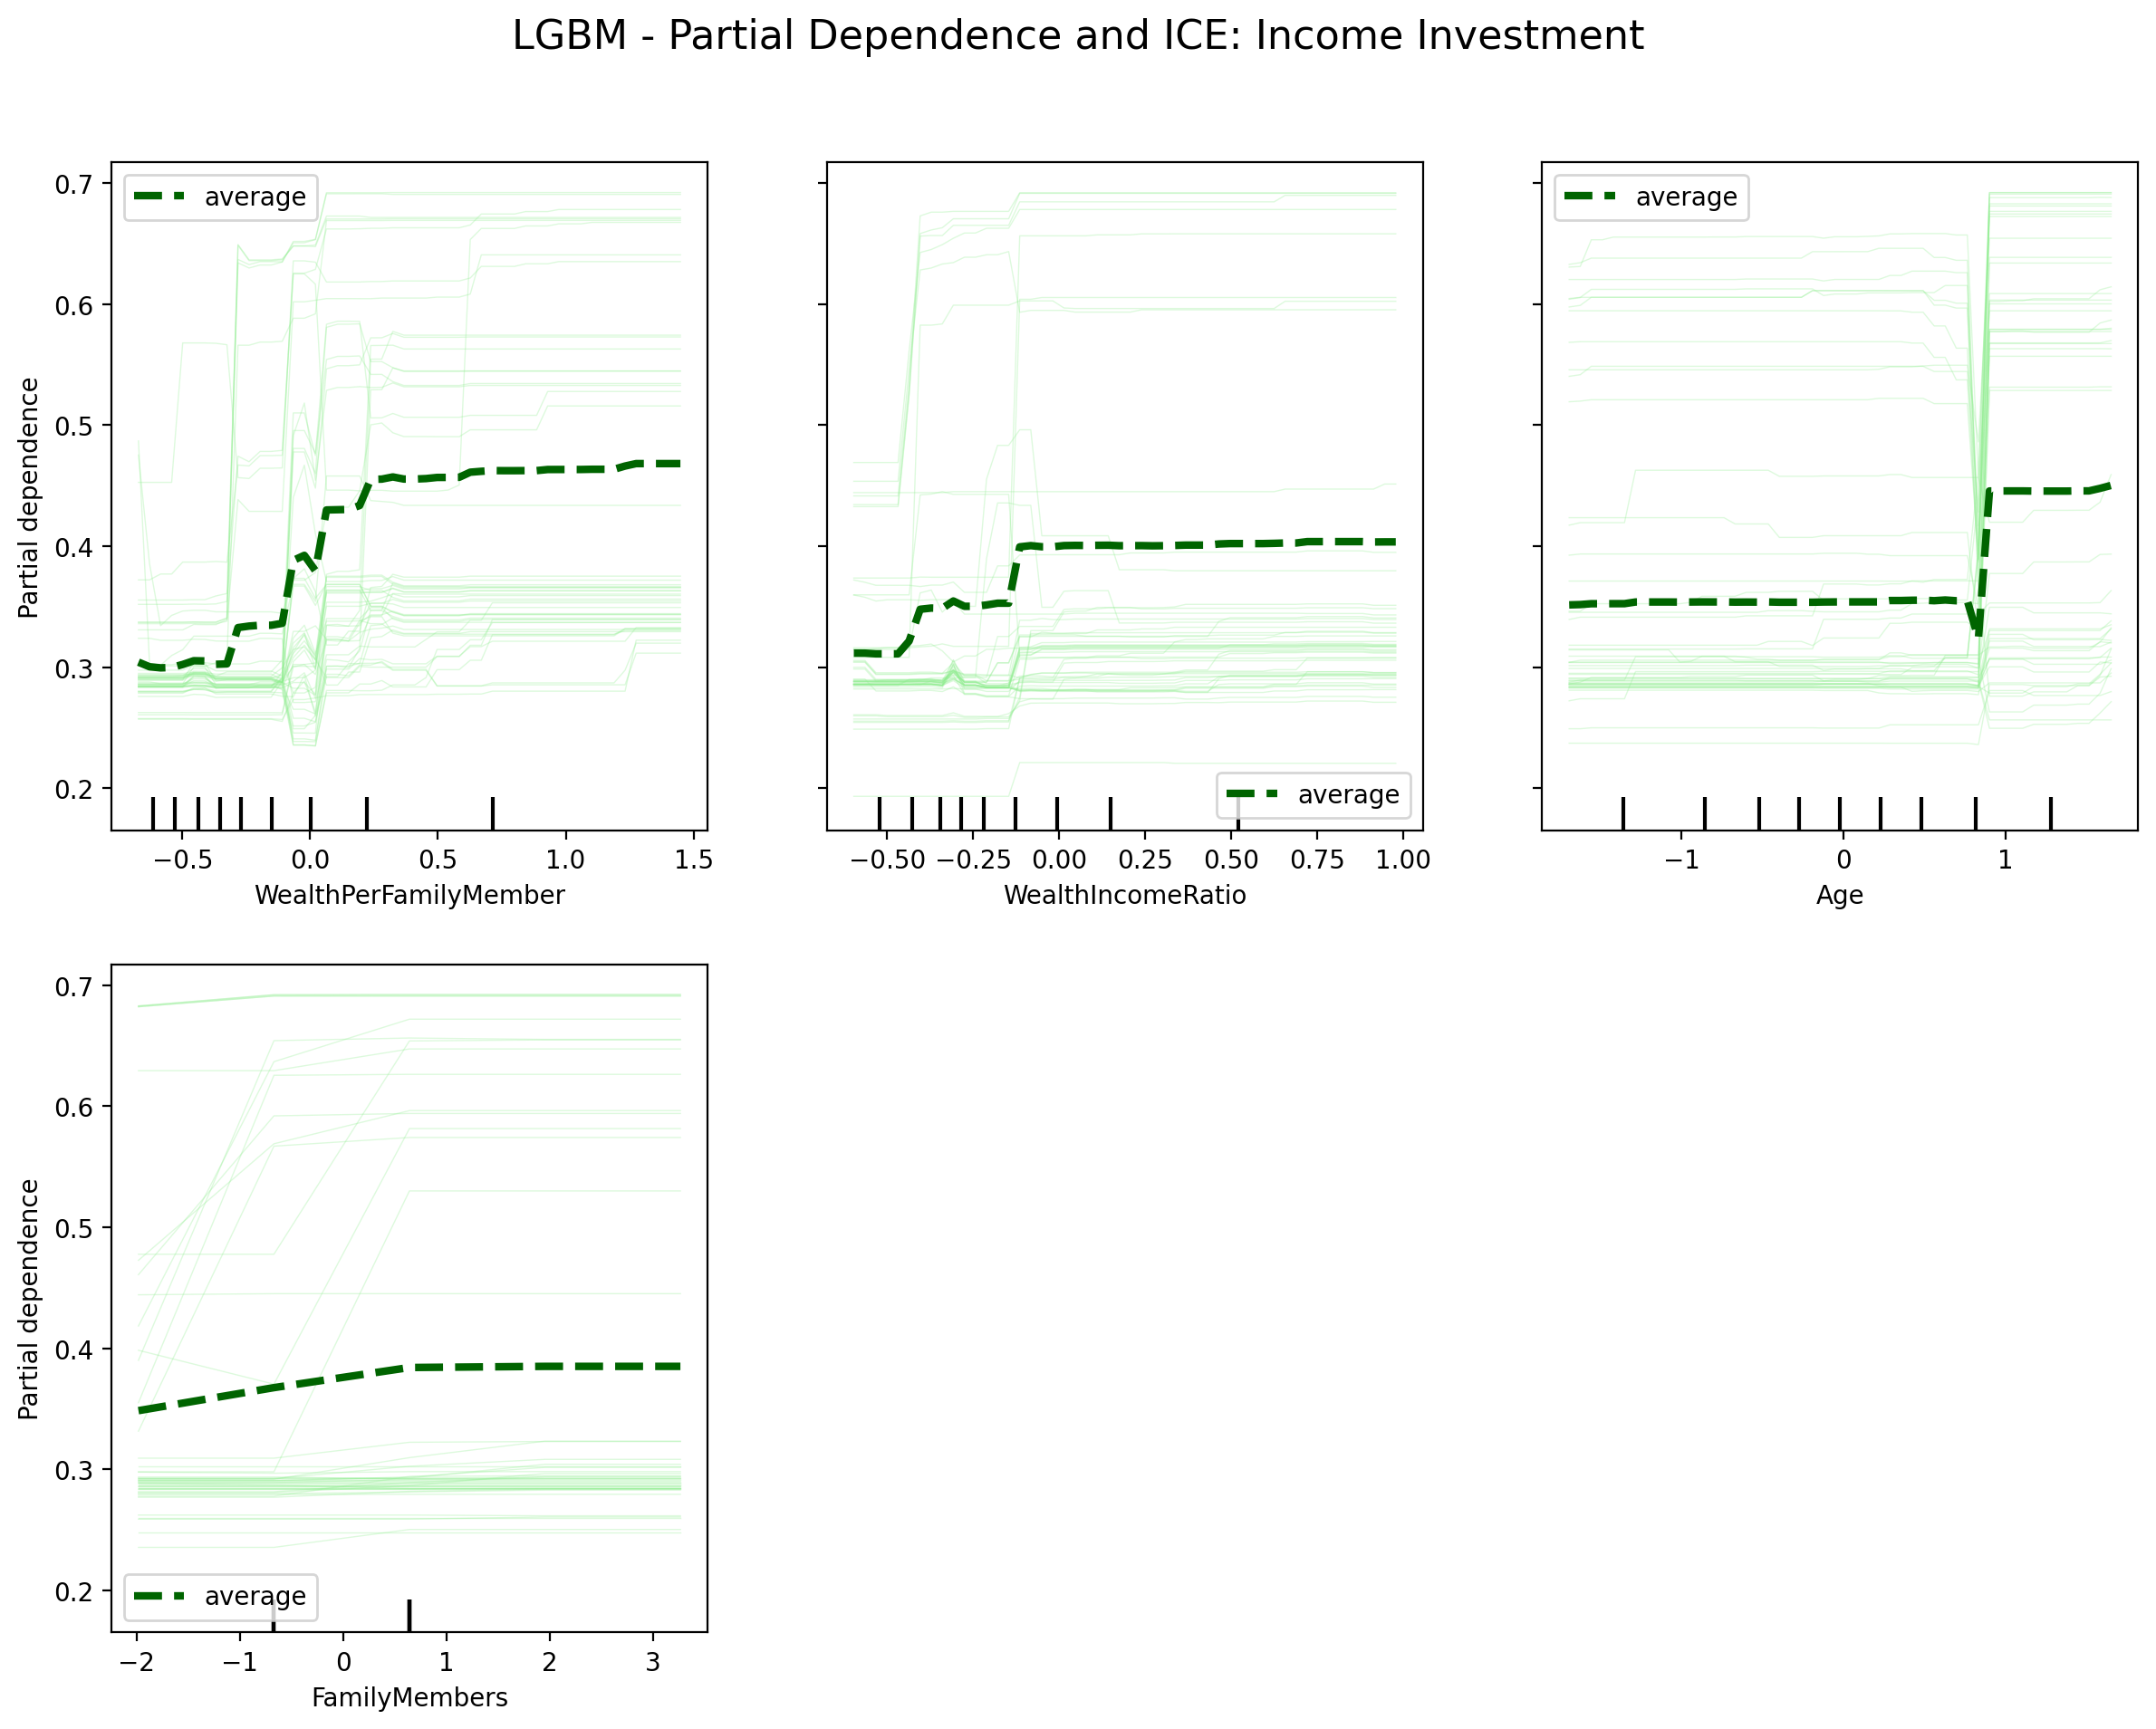
\includegraphics[width=0.7\textwidth,height=0.65\textheight,keepaspectratio]{figures/extracted_img_13.png}\\
	\small \textit{Example LIME Explanation for a single client prediction (LightGBM Income Model)}
\end{frame}

\section{Deep Learning Approach}

\begin{frame}
	\frametitle{Deep Learning Model Architecture: DCN \cite{guo_explainable_2023}}
	\begin{columns}
		\begin{column}{0.5\textwidth}
			\centering
			\resizebox{\linewidth}{!}{
				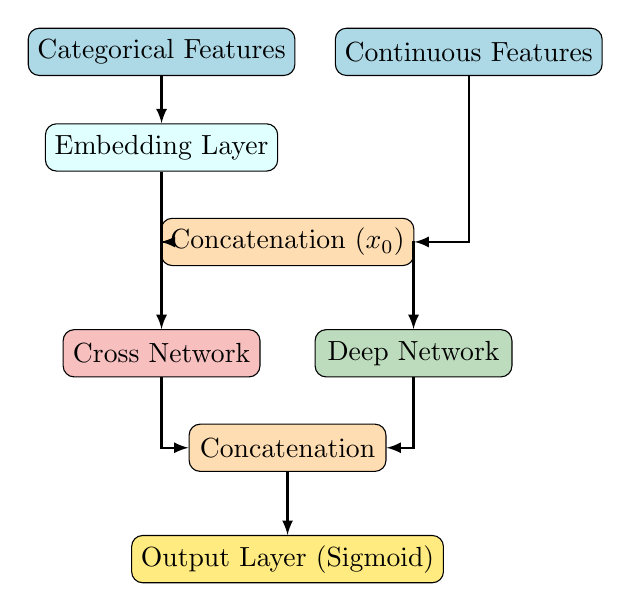
\begin{tikzpicture}[
						box/.style={draw, rounded corners, minimum width=2.5cm, minimum height=0.6cm, align=center},
						arrow/.style={-latex, thick}
					]

					% Inputs
					\node[box, fill=lightblue] (cat) {Categorical Features};
					\node[box, fill=lightblue, right=0.5cm of cat] (cont) {Continuous Features};

					% Embedding
					\node[box, fill=lightcyan, below=0.6cm of cat] (embed) {Embedding Layer};

					% Concat
					\node[box, fill=orange!30, below=1.8cm of cat, xshift=1.6cm] (concat) {Concatenation ($x_0$)};

					% Two paths
					\node[box, fill=lightcoral!50, below=0.8cm of concat, xshift=-1.6cm] (cross) {Cross Network};
					\node[box, fill=darkgreen!30, below=0.8cm of concat, xshift=1.6cm] (deep) {Deep Network};

					% Concat 2
					\node[box, fill=orange!30, below=2cm of concat] (concat2) {Concatenation};

					% Output
					\node[box, fill=gold!50, below=0.8cm of concat2] (out) {Output Layer (Sigmoid)};

					% Arrows
					\draw[arrow] (cat) -- (embed);
					\draw[arrow] (embed) |- (concat);
					\draw[arrow] (cont) |- (concat);

					\draw[arrow] (concat) -| (cross);
					\draw[arrow] (concat) -| (deep);

					\draw[arrow] (cross) |- (concat2);
					\draw[arrow] (deep) |- (concat2);

					\draw[arrow] (concat2) -- (out);
				\end{tikzpicture}
			}
		\end{column}
		\begin{column}{0.5\textwidth}
			\textbf{Multi-Task Learning Results}

			\vspace{0.3cm}
			\resizebox{\linewidth}{!}{%
				\begin{tabular}{lccccc}
					\toprule
					\textbf{Task} & \textbf{Acc} & \textbf{Prec} & \textbf{Rec} & \textbf{F1} & \textbf{AUC} \\
					\midrule
					Income        & 0.783        & 0.852         & 0.544        & 0.664       & 0.767        \\
					Accum.        & 0.795        & 0.846         & 0.708        & 0.771       & 0.852        \\
					\bottomrule
				\end{tabular}%
			}

			\vspace{0.6cm}
			\textbf{Architecture Highlights}
			\begin{itemize}
				\item \textbf{Cross Network}: Applies explicit bounded-degree feature crossing efficiently.
				\item \textbf{Deep Network}: Learns implicit non-linear higher-order interactions.
				\item \textbf{Joint Training}: Both networks share the same concatenated input embeddings, optimising for dual investment targets.
			\end{itemize}
		\end{column}
	\end{columns}
\end{frame}

\section{Recommendations}

\begin{frame}
	\frametitle{Methodology: User-Item Matrix}
	We construct a user-item interaction matrix $R$ using predicted probabilities from the supervised classifiers, penalised by risk misalignment.

	\begin{block}{Matrix Entry $R_{ij}$}
		$$
			R_{ij} = P_{\text{type}(j)}(i) \cdot \big(1 - \alpha \cdot | \text{RiskPropensity}(i) - \text{Risk}(j) |\big)
		$$
	\end{block}

	\begin{itemize}
		\item $P_{\text{type}(j)}(i)$: Predicted probability of client $i$ needing product $j$'s type (Accumulation or Income).
		\item $\alpha \in [0,1]$: Decay factor penalising risk misalignment.
		      \begin{itemize}
			      \item \textbf{Economic Rationale}: Reflects the firm's risk aversion and regulatory suitability constraints (e.g., MiFID II).
			      \item \textbf{Trade-off}: Balances maximising expected fee revenue/conversion against minimising compliance risks and long-term customer churn from unsuitable investments.
		      \end{itemize}
	\end{itemize}
\end{frame}

\begin{frame}
	\frametitle{Methodology: Models \& Evaluation}
	We use model-based CF \cite{sharaf_survey_2022} leveraging matrix $R$:

	\begin{itemize}
		\item \textbf{Truncated SVD}: Factorises $R \approx U_k \Sigma_k V_k^T$ into low-dimensional latent factors to capture hidden preferences.
		\item \textbf{Autoencoder}: Learns non-linear representations by compressing and reconstructing the interaction matrix ($z_u = f_\theta(r_u)$, $\hat{r}_u = g_\phi(z_u)$).
	\end{itemize}

	\vspace{0.3cm}
	\textbf{Evaluation Metrics}
	\begin{itemize}
		\item \textbf{RMSE}: Measures the model's reconstruction error.
		\item \textbf{Precision@$k$ \& Recall@$k$}: Evaluate the relevance of the top-$k$ recommendations.
		\item \textbf{NDCG@$k$}: Assesses ranking quality, prioritising relevant items placed higher.
	\end{itemize}
\end{frame}

\begin{frame}
	\frametitle{Experimental Results}

	\begin{table}
		\centering
		\resizebox{0.8\textwidth}{!}{%
			\begin{tabular}{lcccc}
				\toprule
				\textbf{Model} & \textbf{RMSE}  & \textbf{Precision@3} & \textbf{Recall@3} & \textbf{NDCG@3} \\
				\midrule
				Truncated SVD  & 0.402          & 0.937                & 0.937             & 0.952           \\
				Autoencoder    & \textbf{0.039} & \textbf{0.984}       & \textbf{0.984}    & \textbf{0.997}  \\
				\bottomrule
			\end{tabular}%
		}
	\end{table}

	\begin{columns}
		\begin{column}{0.5\textwidth}
			\centering
			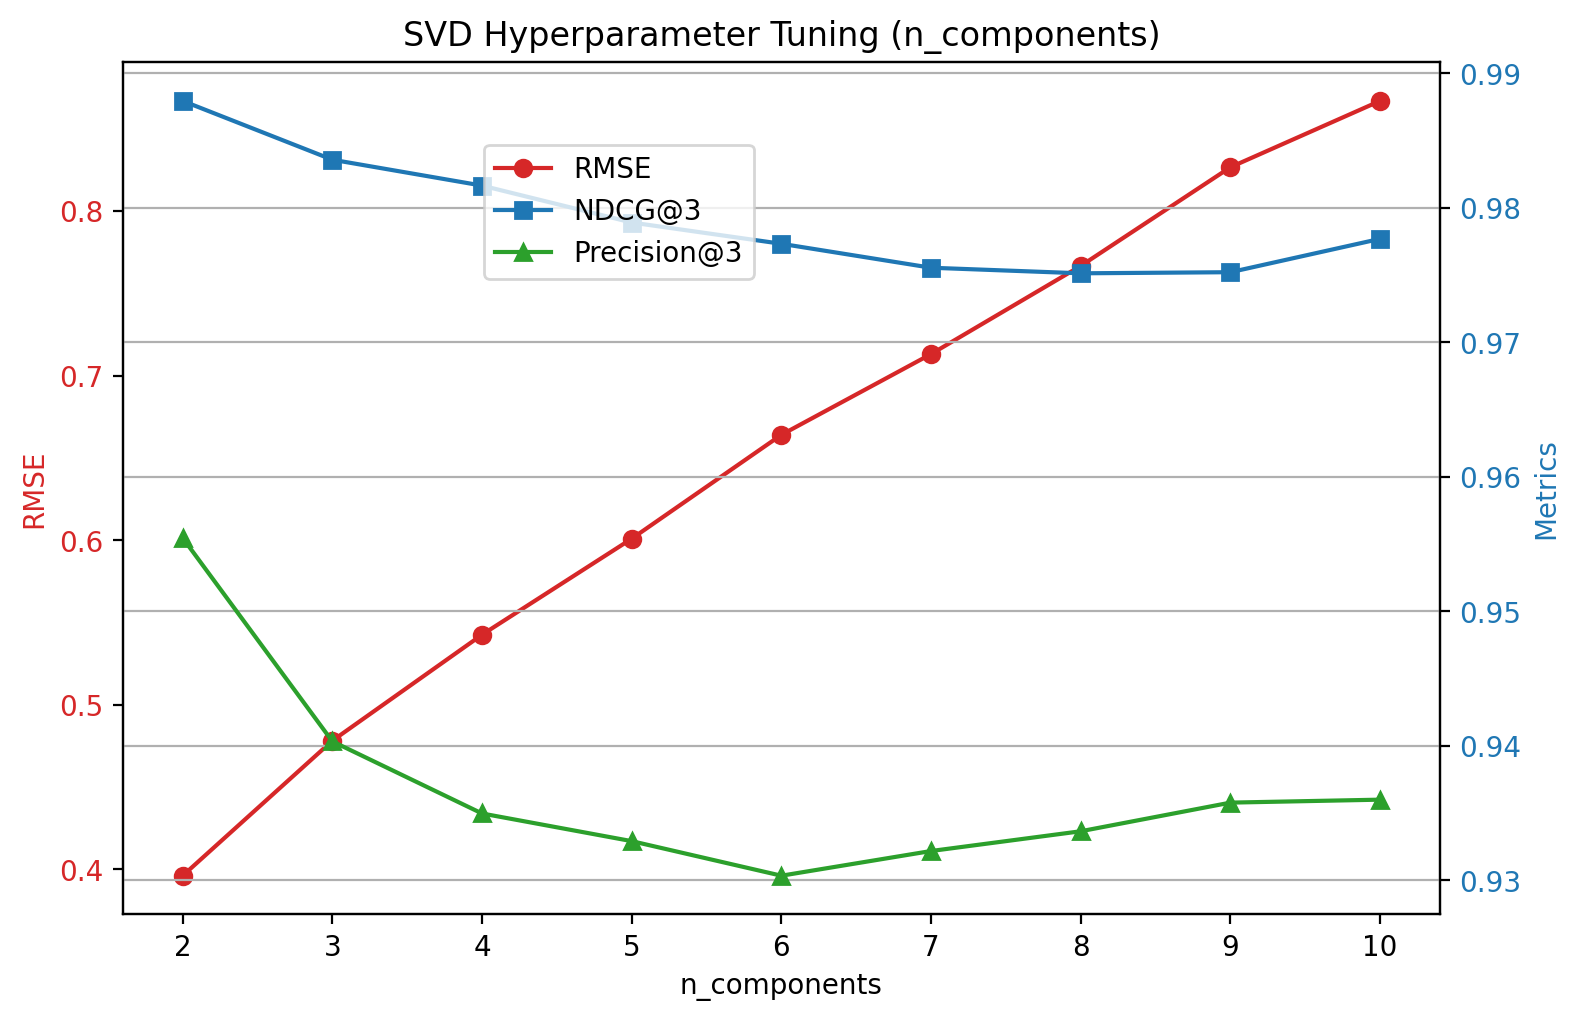
\includegraphics[width=0.8\linewidth]{figures/svd_tuning.png}\\
			\small SVD Tuning
		\end{column}
		\begin{column}{0.5\textwidth}
			\centering
			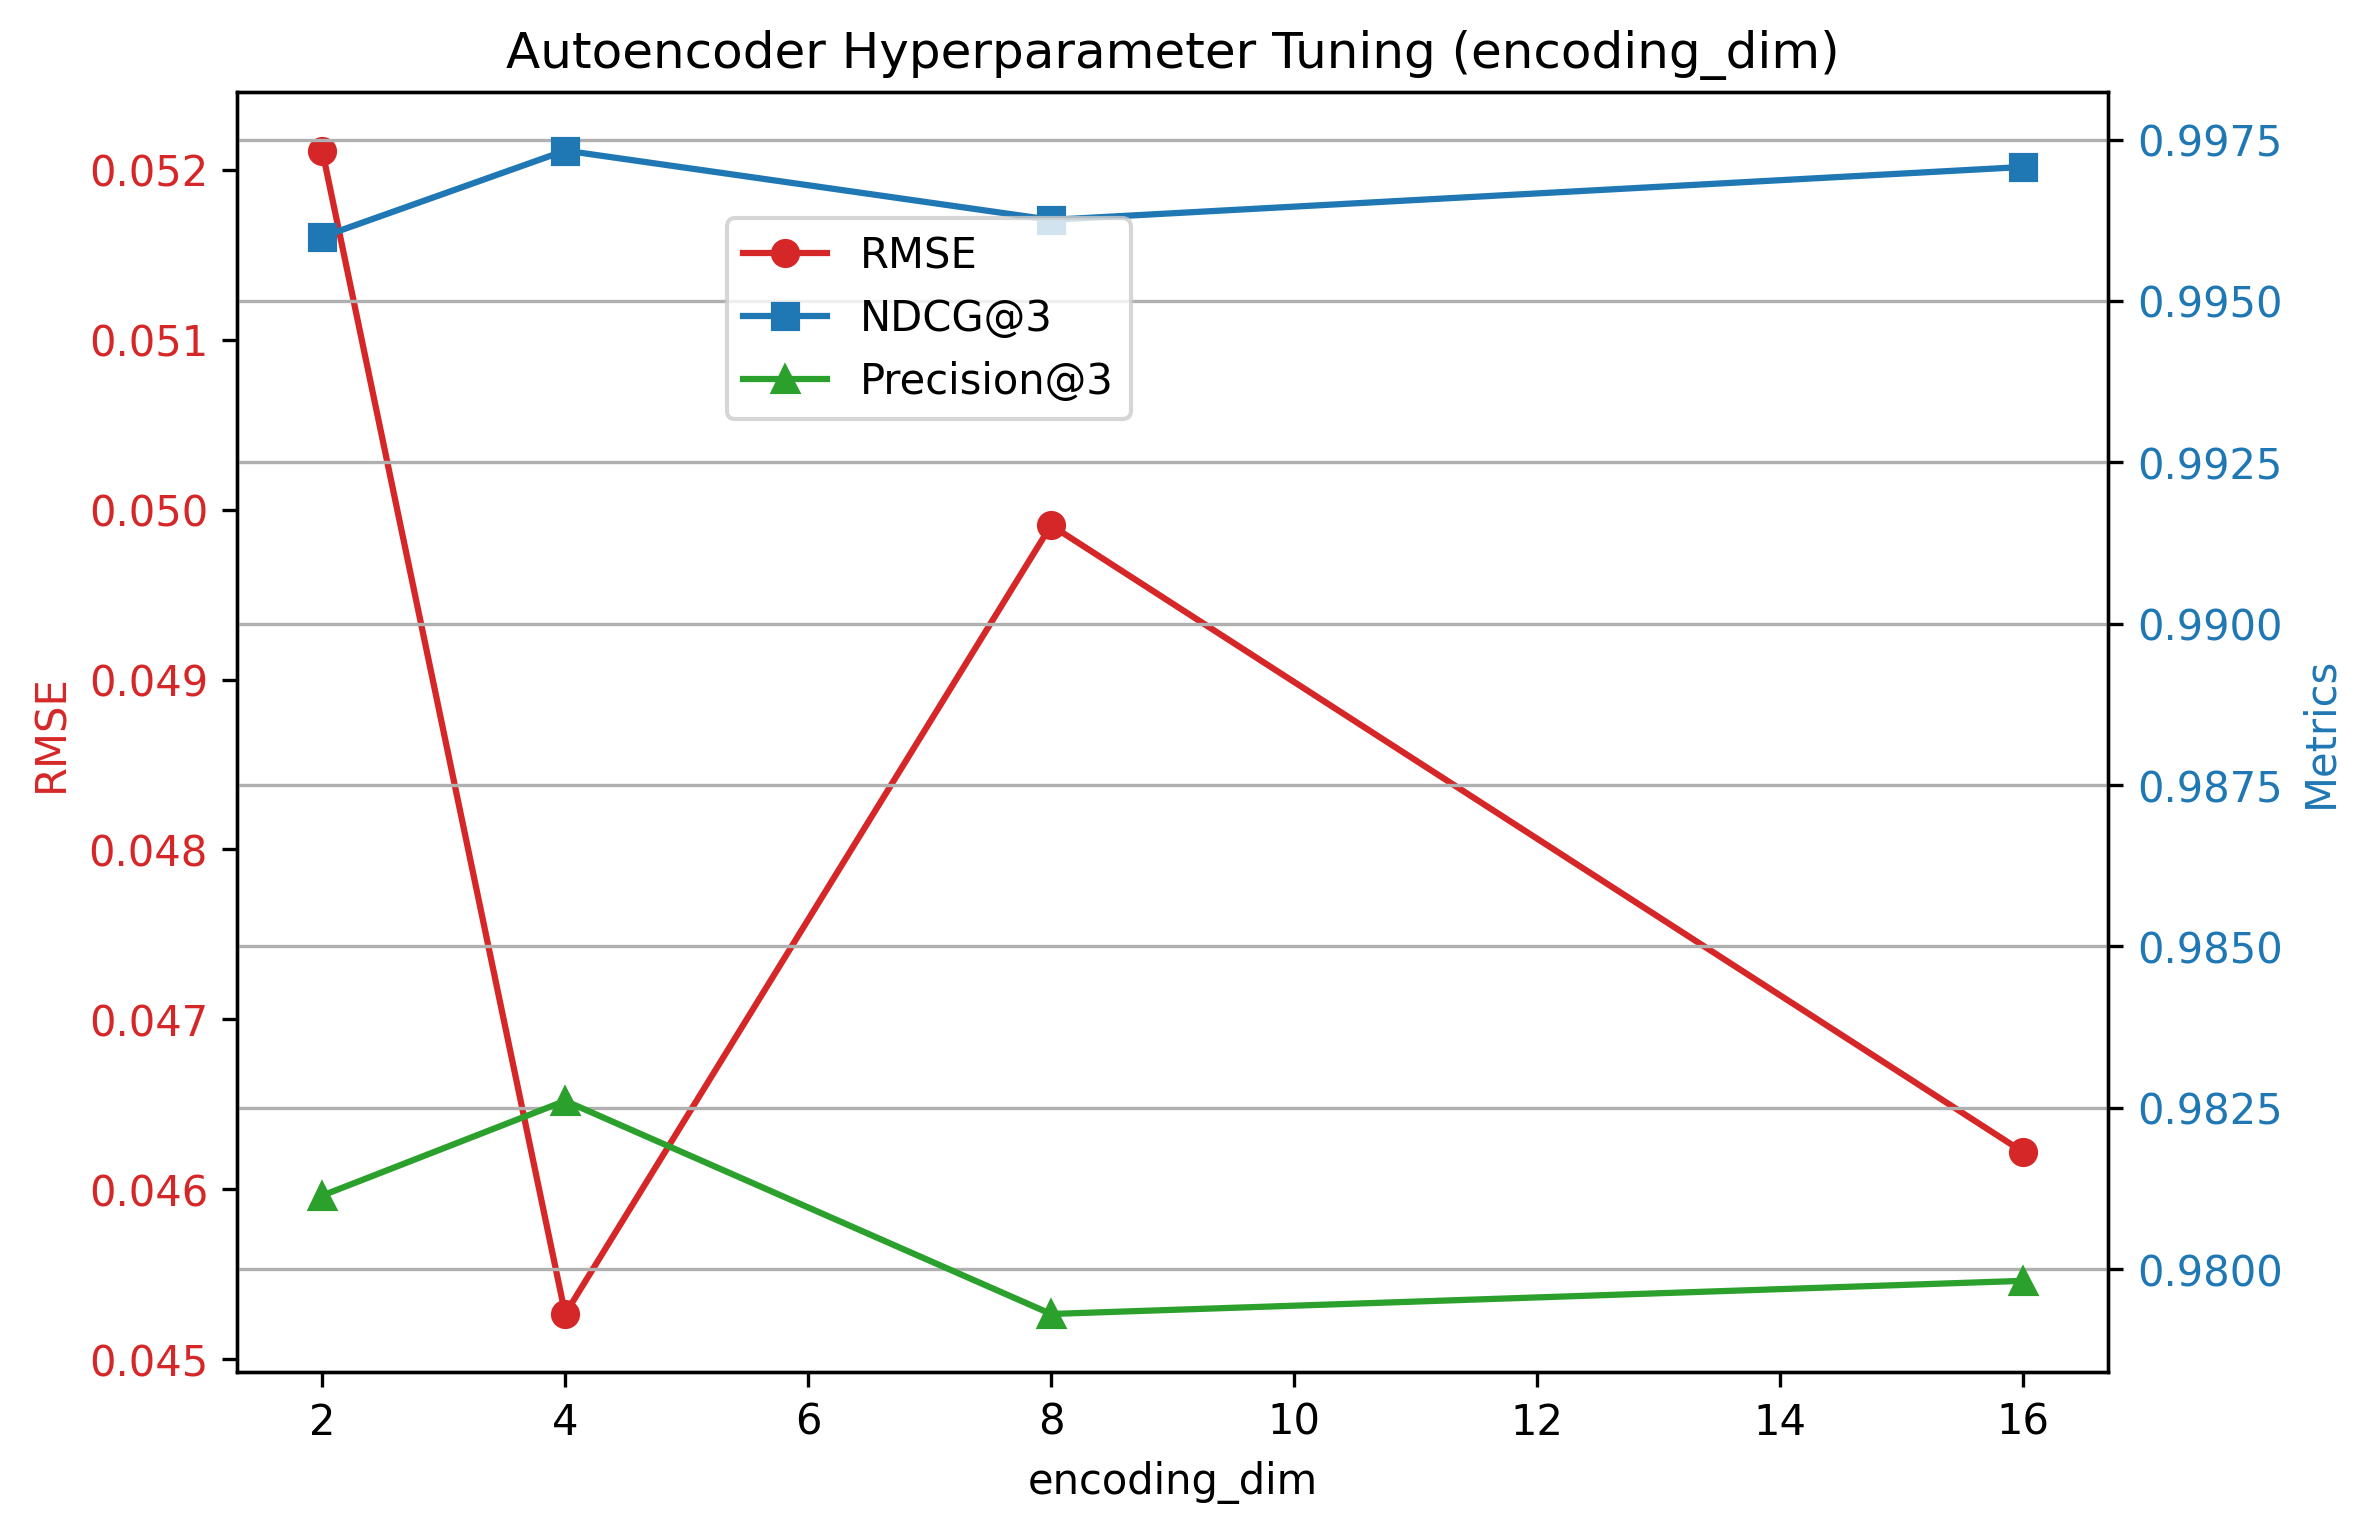
\includegraphics[width=0.8\linewidth]{figures/autoencoder_tuning.png}\\
			\small Autoencoder Tuning
		\end{column}
	\end{columns}
\end{frame}


% =====================================================================
% SECTION 8: CONCLUSION
% =====================================================================
\section{Conclusion}

\begin{frame}
	\frametitle{Project Summary}
	\begin{itemize}
		\item \textbf{Comprehensive ML Pipeline:} Integrated extensive feature engineering, missing value imputation, and log-scaling directly into a robust scikit-learn pipeline to handle skewed financial metrics.
		\item \textbf{Targeted Model Selection:} Selected and optimized LightGBM for the F0.5 score, successfully prioritizing precise, risk-appropriate recommendations over raw recall.
		\item \textbf{Deep Learning Insights:} Leveraged a Deep \& Cross Network (DCN) to learn explicit feature combinations jointly across two prediction tasks.
		\item \textbf{Personalized Recommendations:} Built an Autoencoder-based Collaborative Filtering system that significantly outperforms SVD while enforcing business-driven risk misalignment penalties.
		\item \textbf{Interpretability First:} Embedded global (SHAP) and local (LIME) interpretability, ensuring that every algorithmic recommendation is explainable to financial advisors and regulatory bodies.
	\end{itemize}
\end{frame}

\begin{frame}
	\frametitle{References}
	\printbibliography
\end{frame}

\end{document}
